\documentclass[aspectratio=169,10pt]{beamer}

\usetheme{metropolis}
\usepackage{appendixnumberbeamer}
\usepackage{booktabs}
\usepackage[scale=2]{ccicons}
\usepackage{pgfplots}
\usepgfplotslibrary{dateplot}
\usepackage{xspace}
\usepackage{tikz}
\usetikzlibrary{mindmap,trees,shapes,arrows,positioning,pie}
\usepackage{tcolorbox}

\title{Guide to Pursuing a Computer Science PhD in Europe (Germany Focus)}
\subtitle{Talk 1: Introduction and Preparation}
\date{\today}
\author{Dr. Bijun Li}
\institute{Expert in International Computer Science Research}

\begin{document}

\maketitle

\begin{frame}{About the Speaker: Dr. Bijun Li}
    \begin{columns}[T]
        \begin{column}{0.7\textwidth}
            \textbf{Background}
            \begin{itemize}
                \item PhD in Computer Science from [University Name]
                \item Expert in International Computer Science Research
                \item [X] years of experience in academia and industry
            \end{itemize}
            
            \textbf{Areas of Expertise}
            \begin{itemize}
                \item [Specific area of CS, e.g., Machine Learning, Cybersecurity]
                \item International research collaborations
                \item PhD mentoring and academic career development
            \end{itemize}
            
            \textbf{Notable Achievements}
            \begin{itemize}
                \item [Achievement 1, e.g., Prestigious grant or award]
                \item [Achievement 2, e.g., Key publication or research breakthrough]
                \item [Achievement 3, e.g., Industry partnership or patent]
            \end{itemize}
        \end{column}
%        \begin{column}{0.3\textwidth}
%            % Placeholder for speaker's photo
%            \includegraphics[width=\textwidth]{speaker_photo.jpg}
%        \end{column}
    \end{columns}
\end{frame}

\begin{frame}{Overview}
    \textbf{Talk 1: Introduction and Preparation}
    \begin{itemize}
        \item Introduction to CS PhD programs in Europe
        \item Unique aspects of the German academic system
        \item Preparation for applying
        \item Application process
    \end{itemize}
    
    \textbf{Talk 2: PhD Life and Beyond}
    \begin{itemize}
        \item Funding and financial planning
        \item Starting your PhD and research life
        \item Publishing and conferences
        \item Completing your PhD and career prospects
    \end{itemize}
\end{frame}

\begin{frame}{Introduction: CS PhD Programs in Europe}
    \begin{itemize}
        \item Growing importance of advanced CS research
        \item Europe as a hub for cutting-edge CS PhD programs
        \item Comparison with other global research hubs
    \end{itemize}
    
    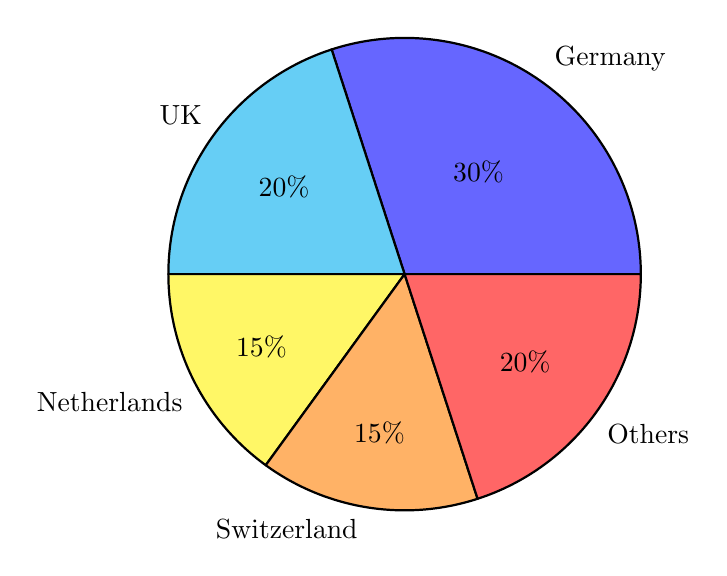
\begin{tikzpicture}
        \pie{30/Germany, 20/UK, 15/Netherlands, 15/Switzerland, 20/Others}
    \end{tikzpicture}
%    \caption{Distribution of top-ranked CS PhD programs in Europe}
\end{frame}

\begin{frame}{Unique Aspects of the German Academic System}
    \begin{itemize}
        \item Strong industry partnerships
        \item Excellent funding opportunities
        \item World-class research institutions
        \item Focus on applied research
        \item Structured vs. individual doctorate programs
    \end{itemize}
\end{frame}

\begin{frame}{Benefits of Pursuing a PhD in Europe/Germany}
    \begin{itemize}
        \item High-quality research environment
        \item International collaboration opportunities
        \item Access to cutting-edge technologies and resources
        \item Strong emphasis on work-life balance
        \item Potential for industry connections
        \item Cultural experience and language skills
    \end{itemize}
\end{frame}

\begin{frame}{Preparation: Prerequisites}
    \textbf{Academic Qualifications}
    \begin{itemize}
        \item Master's degree in CS or related field
        \item Strong academic record (typically 2.0 or better in German grading system)
    \end{itemize}
    
    \textbf{Language Requirements}
    \begin{itemize}
        \item English: Usually IELTS 6.5+ or equivalent
        \item German: Often not required, but beneficial
    \end{itemize}
    
    \textbf{Research Experience}
    \begin{itemize}
        \item Master's thesis
        \item Publications or conference presentations
        \item Relevant internships or projects
    \end{itemize}
\end{frame}

\begin{frame}{Choosing Your Research Area}
    \begin{itemize}
        \item Assess your interests and strengths
        \item Explore current trends in CS research
        \item Consider interdisciplinary opportunities
        \item Align with potential career goals
    \end{itemize}
    
    \textbf{Popular CS Research Areas in Germany}
    \begin{itemize}
        \item Artificial Intelligence and Machine Learning
        \item Cybersecurity and Cryptography
        \item Quantum Computing
        \item Human-Computer Interaction
        \item Big Data and Data Science
    \end{itemize}
\end{frame}

\begin{frame}{Identifying Potential Supervisors and Institutions}
    \textbf{Top CS Universities and Research Institutions}
    \begin{itemize}
        \item Technical University of Munich (TUM)
        \item RWTH Aachen University
        \item Max Planck Institute for Informatics
        \item German Research Center for Artificial Intelligence (DFKI)
    \end{itemize}
    
    \textbf{Finding the Right Supervisor}
    \begin{itemize}
        \item Research faculty profiles and publications
        \item Attend CS conferences and workshops
        \item Leverage online platforms (e.g., ResearchGate, GitHub)
        \item Consider reaching out for informal discussions
    \end{itemize}
\end{frame}

\begin{frame}{PhD Structures in Germany}
    \begin{columns}[T]
        \begin{column}{0.5\textwidth}
            \textbf{Individual Doctorate}
            \begin{itemize}
                \item Traditional model
                \item More flexible structure
                \item Focus on independent research
                \item Often tied to research assistant positions
            \end{itemize}
        \end{column}
        \begin{column}{0.5\textwidth}
            \textbf{Structured Programs}
            \begin{itemize}
                \item More formal curriculum
                \item Includes coursework
                \item Often interdisciplinary
                \item May offer more networking opportunities
            \end{itemize}
        \end{column}
    \end{columns}
    
    \textbf{Choose Based On}
    \begin{itemize}
        \item Your research goals
        \item Preferred work style
        \item Career aspirations
    \end{itemize}
\end{frame}

\begin{frame}{Application Process: Finding PhD Positions}
    \begin{itemize}
        \item University websites and job boards
        \item Online academic job portals
            \begin{itemize}
                \item academics.de
                \item euraxess.ec.europa.eu
                \item jobs.ac.uk
            \end{itemize}
        \item Research institute openings
        \item Professional networks (LinkedIn, ResearchGate)
        \item CS conferences and workshops
    \end{itemize}
    
    \textbf{Tip:} Set up job alerts on these platforms to stay updated on new openings
\end{frame}

\begin{frame}{Preparing Application Materials}
    \begin{columns}[T]
        \begin{column}{0.5\textwidth}
            \textbf{CV/Resume}
            \begin{itemize}
                \item Academic background
                \item Research experience
                \item Technical skills
                \item Publications/presentations
            \end{itemize}
            
            \textbf{Research Proposal}
            \begin{itemize}
                \item Clear research question
                \item Methodology
                \item Potential impact
                \item Alignment with supervisor/program
            \end{itemize}
        \end{column}
        \begin{column}{0.5\textwidth}
            \textbf{Letters of Recommendation}
            \begin{itemize}
                \item From academic/research supervisors
                \item Highlighting research potential
            \end{itemize}
            
            \textbf{Transcripts and Certificates}
            \begin{itemize}
                \item Academic records
                \item Degree certificates
                \item Language proficiency proof
            \end{itemize}
        \end{column}
    \end{columns}
\end{frame}

\begin{frame}{Application Timelines and Interview Process}
    \textbf{Timelines}
    \begin{itemize}
        \item Vary by institution and program
        \item Generally, 6-12 months before intended start date
        \item Some programs have fixed annual deadlines
        \item Others review applications on a rolling basis
    \end{itemize}
    
    \textbf{Interview Process}
    \begin{itemize}
        \item Often conducted via video call
        \item May include presentation of past research/proposal
        \item Questions on technical knowledge and research interests
        \item Discussion of program expectations and your goals
    \end{itemize}
    
    \textbf{Tip:} Prepare a short "elevator pitch" about your research interests
\end{frame}

\begin{frame}{Q\&A Session}
    \centering
    \large{Time for Your Questions!}
    
    \vspace{1cm}
    
    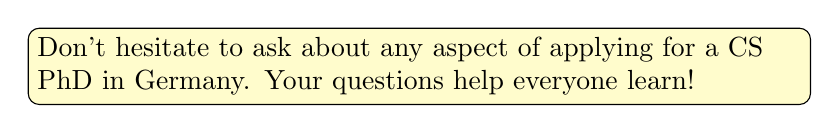
\begin{tikzpicture}
        \node[draw,rounded corners,fill=yellow!20,text width=0.8\textwidth] {
            Don't hesitate to ask about any aspect of applying for a CS PhD in Germany. Your questions help everyone learn!
        };
    \end{tikzpicture}
\end{frame}

\begin{frame}{Preview of Talk 2 and Homework}
    \textbf{Coming Up in Talk 2}
    \begin{itemize}
        \item Funding and financial planning
        \item Starting your PhD and research life
        \item Publishing and attending conferences
        \item Completing your PhD and career prospects
    \end{itemize}
    
    \textbf{Homework}
    \begin{itemize}
        \item Research 2-3 potential CS PhD programs or research groups in Germany
        \item Draft an initial research proposal in your area of interest
        \item Identify key CS conferences in your subfield and their deadlines
        \item Prepare questions about funding and PhD life for next session
    \end{itemize}
\end{frame}

\end{document}